\documentclass[12pt,a4paper]{article} 

\usepackage{titlesec}
\usepackage{color}
\usepackage[utf8]{inputenc}
\usepackage[english]{babel}
\usepackage[T1]{fontenc}
\usepackage{graphicx}
\graphicspath{{Images/}}
\usepackage{eso-pic} 
\usepackage{subfig} 
\usepackage{caption} 
\usepackage{transparent}
\usepackage{amsmath}
\usepackage{amsthm}
\usepackage{bm}
\usepackage[overload]{empheq}  
\usepackage{tabularx}
\usepackage{longtable}
\usepackage{colortbl}
\usepackage{algorithm}
\usepackage{algorithmic}
\usepackage[colorlinks=true,linkcolor=black,anchorcolor=black,citecolor=black,filecolor=black,menucolor=black,runcolor=black,urlcolor=black]{hyperref} 
\usepackage{cleveref}
\usepackage[square, numbers, sort&compress]{natbib} 
\bibliographystyle{plain} 
\usepackage{appendix}
\usepackage{enumitem}
\usepackage{amsthm,thmtools,xcolor} 
\usepackage{comment} 
\usepackage{fancyhdr} 
\usepackage{lipsum} 
\usepackage{tcolorbox} 
\newcommand{\bea}{\begin{eqnarray}} 
\newcommand{\eea}{\end{eqnarray}}
\newcommand{\e}[1]{\times 10^{#1}}  
\newcommand{\mathbbm}[1]{\text{\usefont{U}{bbm}{m}{n}#1}} 
\newcommand{\pdev}[2]{\frac{\partial#1}{\partial#2}}

% Configuration package
\usepackage[bottom=2.0cm,top=2.0cm,left=2.0cm,right=2.0cm]{geometry}
\raggedbottom 

% Create color bluePoli (-> manuale grafica coordinata:  https://www.polimi.it/fileadmin/user_upload/il_Politecnico/grafica-coordinata/2015_05_11_46xy_manuale_grafica_coordinata.pdf)
\definecolor{bluePoli}{cmyk}{0.4,0.1,0,0.4}

% Custom theorem environments
\declaretheoremstyle[
  headfont=\color{bluePoli}\normalfont\bfseries,
  bodyfont=\color{black}\normalfont\itshape,
]{colored}

\captionsetup[figure]{labelfont={color=bluePoli}} % Set colour of the captions
\captionsetup[table]{labelfont={color=bluePoli}} % Set colour of the captions
\captionsetup[algorithm]{labelfont={color=bluePoli}} % Set colour of the captions

\theoremstyle{colored}
\newtheorem{theorem}{Theorem}[section]
\newtheorem{proposition}{Proposition}[section]

% Enhances the features of the standard "table" and "tabular" environments.
\newcommand\T{\rule{0pt}{2.6ex}}
\newcommand\B{\rule[-1.2ex]{0pt}{0pt}}

% Algorithm description
\newcounter{algsubstate}
\renewcommand{\thealgsubstate}{\alph{algsubstate}}
\newenvironment{algsubstates}{
    \setcounter{algsubstate}{0}%
    \renewcommand{\STATE}{%
    \stepcounter{algsubstate}%
    \Statex {\small\thealgsubstate:}\space}
    }{}
    
% Custom theorem environment
\newcolumntype{L}[1]{>{\raggedright\let\newline\\\arraybackslash\hspace{0pt}}m{#1}}
\newcolumntype{C}[1]{>{\centering\let\newline\\\arraybackslash\hspace{0pt}}m{#1}}
\newcolumntype{R}[1]{>{\raggedleft\let\newline\\\arraybackslash\hspace{0pt}}m{#1}}

% Custom itemize environment
\setlist[itemize,1]{label=$\bullet$}
\setlist[itemize,2]{label=$\circ$}
\setlist[itemize,3]{label=$-$}
\setlist{nosep}

% Create command for background pic
\newcommand\BackgroundPic{% Adding background picture
	\put(237,365){
	    \parbox[b][\paperheight]{\paperwidth}{%
	    \vfill
		\centering
		\transparent{0.4}
		
\includegraphics[width=0.44\paperwidth]{raggiera_polimi.eps}%
		\vfill}
		}
}

% Set indentation
\setlength\parindent{0pt}

% Custom title commands
\titleformat{\section}
{\color{bluePoli}\normalfont\Large\bfseries}
{\color{bluePoli}\thesection.}{1em}{}
\titlespacing*{\section}
{0pt}{3.3ex}{3.3ex}

\titleformat{\subsection}
{\color{bluePoli}\normalfont\large\bfseries}
{\color{bluePoli}\thesubsection.}{1em}{}
\titlespacing*{\subsection}
{0pt}{3.3ex}{3.3ex}

% Custom headers and footers
\pagestyle{fancy}
\fancyhf{}
      
\fancyfoot{}
\fancyfoot[C]{\thepage} % page
\renewcommand{\headrulewidth}{0mm} % headrule width
\renewcommand{\footrulewidth}{0mm} % footrule width

\makeatletter
\patchcmd{\headrule}{\hrule}{\color{black}\hrule}{}{} % headrule
\patchcmd{\footrule}{\hrule}{\color{black}\hrule}{}{} % footrule
\makeatother

% -> title of your work
\renewcommand{\title}{KANs: Kolmogorov-Arnold Networks}
% -> author name and surname
\renewcommand{\author}{Pasqual Matteo Romilio}
% -> MSc course
\newcommand{\course}{Master's degree in Computer Science Engineering }
% -> advisor name and surname
\newcommand{\advisor}{Prof. Edie Miglio}
% -> author ID
\newcommand{\ID}{10765765}
% -> academic year
\newcommand{\YEAR}{2024-2025}
% -> abstract (only in English)
\renewcommand{\abstract}{Here goes Abstract }

% -> key-words (only in English)
\newcommand{\keywords}{}

%------------------
%	BEGIN OF YOUR DOCUMENT
%------------------
\begin{document}
% DO NOT REMOVE SPACES BETWEEN LINES!

\AddToShipoutPicture*{\BackgroundPic}

\hspace{-0.6cm}
\includegraphics[width=0.6\textwidth]{logo_polimi_ing_indinf.eps}

\vspace{-1mm}
\Large{\textbf{\color{bluePoli}{\title}}}\\

\vspace{-0.2cm}
\fontsize{0.3cm}{0.5cm}\selectfont \bfseries \textsc{\color{bluePoli}  Project of Numerical Analysis for Machine Learning \\ \course}\\

\vspace{-0.2cm}
\large{\textbf{\author, \ID}}

\small \normalfont

\vspace{11pt}

\centerline{\rule{1.0\textwidth}{0.4pt}}

\begin{center}
\begin{minipage}[t]{.26\textwidth}
\begin{minipage}{.90\textwidth}
\noindent
\scriptsize{\textbf{Advisor:}} \\
\advisor \\
\\ % leave it if any co-advisor otherwise comment
\textbf{Academic year:} \\
\YEAR \\
\\
\end{minipage}
\end{minipage}% This must go next to `\end{minipage}`
\begin{minipage}{.74\textwidth}
\noindent \textbf{\color{bluePoli} Abstract:} {\abstract}
\end{minipage}
\end{center}

\vspace{15pt}

\begin{tcolorbox}[arc=0pt, boxrule=0pt, colback=bluePoli!60, width=\textwidth, colupper=white]
    \textbf{} \keywords
\end{tcolorbox}

\vspace{12pt}

%--------------
% INTRODUCTION
%--------------
\section{Introduction}
\label{sec:in}
Multi-layer perceptrons (MLPs), also known as fully-connected feedforward neural networks, are foundational building blocks of today’s deep learning models. The importance of MLPs can never be overstated, since they are the default models in machine learning for approximating non-linear functions, due to their expressive power guaranteed by the universal approximation theorem. 

However, are MLPs the best non-linear regressors we can build? Despite the prevalent use of MLPs, they have significant drawbacks. In transformers, for example, MLPs consume almost all non-embedding parameters and are typically less interpretable (relative to attention layers) without post-analysis tools.

We propose a promising alternative to MLPs, called Kolmogorov-Arnold Networks (KANs). 

Whereas MLPs are inspired by the universal approximation theorem, KANs are inspired by the Kolmogorov-Arnold representation theorem. Like MLPs, KANs have fully-connected structures. However, while MLPs place fixed activation functions on nodes “neurons”), KANs place learnable activation functions on edges (“weights”), as illustrated in Figure~\ref{fig:MLPKAN}. As a result, KANs have no linear weight matrices at all: instead, each weight parameter is replaced by a learnable 1D function parametrized as a spline. KANs’ nodes simply sum incoming signals without applying any non-linearities. 

One might worry that KANs are hopelessly expensive, since each MLP’s weight parameter becomes KAN’s spline function. Fortunately, KANs usually allow much smaller computation graphs than MLPs embedding a 2-hidden-layer neural network.

Throughout this paper, we will show that KANs can lead to higher accuracy and improved interpretability over MLPs. We will show how, by leveraging the Kolmogorov-Arnold representation theorem, learnable activation functions and the absence of fixed-weight matrices allow KANs to efficiently capture complex relationships within the data\cite{KAN}.

\begin{figure}[H]
    \centering
    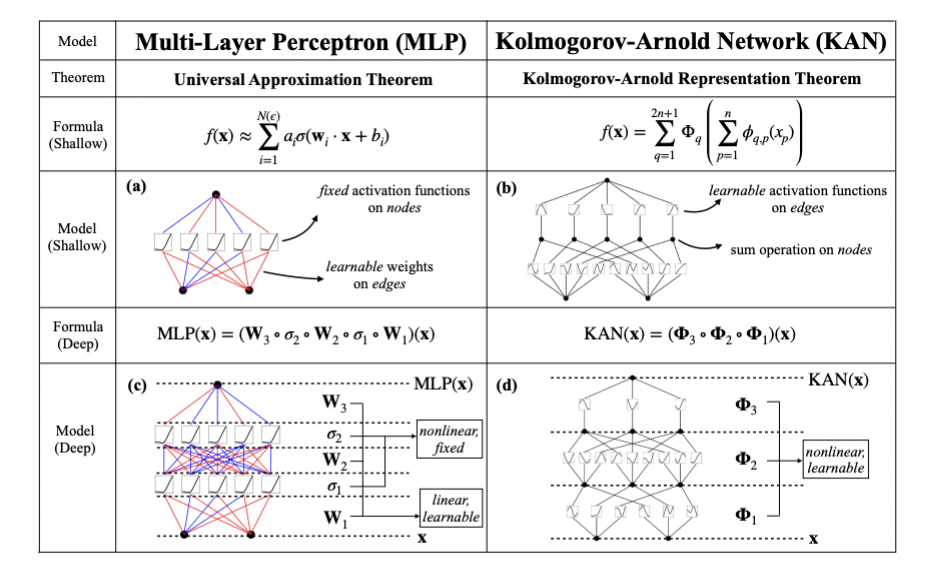
\includegraphics[width=0.8\linewidth]{Images/MLP-KAN.png}
    \caption{Multi-layer perceptrons (MLPs) vs Kolmogorov-Arnold Networks (KANs)}
    \label{fig:MLPKAN}
\end{figure}

%--------------
% Kolmogorov-Arnold
%--------------
\section{Kolmogorov-Arnold representation theorem}
\label{sec:ka}
Whereas Multi-layer perceptrons (MLPs) are inspired by the universal approximation theorem, Kolmogorov-Arnold Networks (KANs) are inspired by the Kolmogorov-Arnold representation theorem \cite{KAN}.

Firstly, we start with the basic concept that a neural network can be described as a multivariate continuous function $f: \Re^n \rightarrow \Re^m $ that maps an input vector $\textbf{x}\in \Re^n$ to an output vector $\textbf{y}\in \Re^m$ via a series of computations. In particular, both MLPs and KANs can be described as a multivariate continuous function $f: \Re^n \rightarrow \Re $ that maps an input vector $\textbf{x}\in \Re^n$ to an output value $y\in \Re$ via a series of computations \cite{book1NAML, book2NAML}.

As in MLP when input variables are combined linearly we have to standardize inputs passing from a domain $D \subset \Re^n$ to a compact domain $D \subset [0,1]^n $. A possibility is to apply an affine transformation to the data so that each feature will be normalized in $[0,1] \in 
 \Re$.

We can now formally present and demonstrate the Kolmogorov-Arnold representation theorem. 

The Kolmogorov-Arnold representation theorem is essential for proving that any neural network that has one output (for instance MLPs) can always be rebuilt as two-hidden-layer KANs. In particular, the Kolmogorov-Arnold representation theorem states that if $f$ is a multivariate continuous function on a bounded domain, then it can be written as a finite composition of continuous functions of a single variable and the binary operation of addition \cite{KAtheorem, KArevisited}.

\begin{theorem}[Kolmogorov-Arnold representation theorem \cite{KAtheorem}] 
\label{Kolmogorov-Arnold}
Let $f$ be an arbitrary multivariate continuous function on a bounded domain $f:[0,1]^n -> \Re$, then $f$:

$$f(\textbf{x}) = f(x_1,x_2,...,x_n) = \sum_{q=1}^{2n+1} \Phi_q(\sum_{p=1}^n \phi_{q,p}(x_p))$$

with continuous one–dimensional inner functions $\phi_{q,p}:[0,1] -> \Re$ and continuous one–dimensional outer functions $\Phi_q:\Re -> \Re$.
\end{theorem} 

In a sense, they showed that the only true multivariate function is addition since every other function can be written using univariate functions and sum. The great advantage is that we have to learn only a polynomial number of 1D functions. However, these 1D functions can be non-smooth and even fractal, so they may not be learnable; in practice with spline function, we can approximate their shapes and achieve the accuracy that we want \cite{KAN}.

\subsection{Matrix form}
For a better representation, the Kolmogorov-Arnold representation of $f: [0,1]^n \rightarrow \Re$ can be written in matrix form \cite{KAN}:

$$f(\textbf{x}) = \boldsymbol{\Phi_{out}} \times \boldsymbol{\Phi_{in} }\times \textbf{x}$$

where $\textbf{x} \in \Re^n$, $\boldsymbol{\Phi_{in}} \in \Re^{2n+1,n}$, and $\boldsymbol{\Phi_{out}} \in \Re^{2n+1}$:

\[
\boldsymbol{\Phi_{in}} = 
\begin{pmatrix}
\phi_{1,1}(\cdot) & \dots & \phi_{1,n}(\cdot) \\
\vdots &   & \vdots \\
\phi_{2n+1,1}(\cdot) & \dots & \phi_{2n+1,n}(\cdot)
\end{pmatrix},
\quad \boldsymbol{\Phi_{in}} = (\Phi_{1}(\cdot) \dots \Phi_{2n+1}(\cdot))
\]

We can notice that both $\boldsymbol{\Phi_{in}}$ and $\boldsymbol{\Phi_{out}}$ are special cases of the following function matrix $\boldsymbol{\Phi}$ that represent a general Kolmogorov-Arnold layer. 

\[
\boldsymbol{\Phi} = 
\begin{pmatrix}
\phi_{1,1}(\cdot) & \dots & \phi_{1,n_{in}}(\cdot) \\
\vdots &   & \vdots \\
\phi_{n_{out},1}(\cdot) & \dots & \phi_{n_{out},n_{in}}(\cdot)
\end{pmatrix}
\]


Each layer has $n_{in}$ inputs and $n_{out}$ outputs then in our case, the two layers are defined as follows:
\begin{itemize}
    \item Layer 1: $\boldsymbol{\Phi_{in}}$ has $\boldsymbol{\Phi}$ with $n_{in} = n$ and $n_{out} = 2n+1$
    \item Layer 2: $\boldsymbol{\Phi_{out}}$ has $\boldsymbol{\Phi}$ with $n_{in} = 2n+1$ and $n_{out} = 1$
\end{itemize}

\section{KAN Structure}
Kolmogorov-Arnold networks require at least two layers, with a corrective depth of \(2n+1\) and \(n\). However, in practice, we can design larger networks with various structures beyond this minimum requirement \cite{KAN}.

\section{Splines functions}


%--------------
% CONCLUSION
%--------------
\section{Conclusions}

%--------------
% END
%--------------
\bibliography{bibliography.bib}
\end{document}